%! Author = russell
%! Date = 4/11/25

% Preamble
\documentclass[12pt]{article}

% Packages
\usepackage[letterpaper,margin=1in]{geometry}
\usepackage{amsmath}
\usepackage{amsthm}
\usepackage{amsfonts}
\usepackage{amssymb}
\usepackage{fancyhdr}
\usepackage{mathtools}
\usepackage{tikz-cd}
\usepackage{stmaryrd}
\usepackage{enumerate}
\usepackage{capt-of}
\usepackage{xurl}
\usepackage{hyperref}


% Document
\begin{document}
    \setlength{\parindent}{0pt}
    \setlength{\parskip}{5pt}
    \setlength{\headheight}{14.49999pt}
    \addtolength{\topmargin}{-1.59999pt}

    \section*{The Layup Sequence: Three Implementations}

    The \textit{Layup Sequence} is defined as follows:
    \[
        S(n) =
        \begin{cases}
            1 & n = 1 \\
            2 & n = 2 \\
            S(n - 1) + S(n - 2) & n \equiv 0 \pmod{2} \\
            2S(n - 1) - S(n - 2) & n \equiv 1 \pmod{2} \\
        \end{cases}
    \]

    I implemented the function $S$ in three different ways, each with a different time complexity.

    I used Python for its support of large integers and data plotting.
    I would prefer to work in Rust, but I have not used large integer or data plotting
    libraries in Rust before and did not want to learn them right now.
    I could prove the correctness of the algorithms in Lean, but that would
    take much longer to write, and would be out of the scope of the assignment,
    and would be unfair to force Mr. Bonecutter or anyone else on the hiring team to read.

    Throughout the report I treat the cost of multiplying integers as constant,
    but it theoretically should become significant for large values of $n$
    for which the binary exponentiation algorithm is still feasible,
    and may account for some of the data distribution.

    \subsection*{The Naive Implementation}

    The naive implementation recursively calls itself as is explicit in the specification.
    Since each function call results in two function calls,
    the time complexity is exponential.
    (It technically has a different base from $O(2^n)$,
    but for all practical purposes it can be considered the same.)

    The runtimes for $n \in \{2, 4, \dots, 20\}$
    when run $1000$ times each make the following plot:

    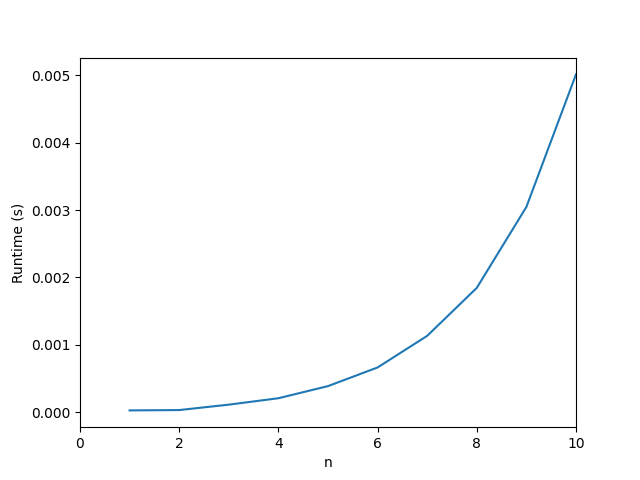
\includegraphics[scale=0.65]{naive}

    This indeed appears to be an exponential relation.

    \subsection*{The Iterative Implementation}

    The iterative implementation avoids recalculating the same value of $S(i)$ for any particular $i$
    by iteratively calculating $(S(i), S(i + 1))$ in terms of $(S(i - 1), S(i))$.
    Since it simply loops for $i$ up to $n$ and each loop is just arithmetic,
    the time complexity is $O(n)$.

    The runtimes for $n \in \{1000, 2000, \dots, 10000\}$
    when run $1000$ times each make the following plot:

    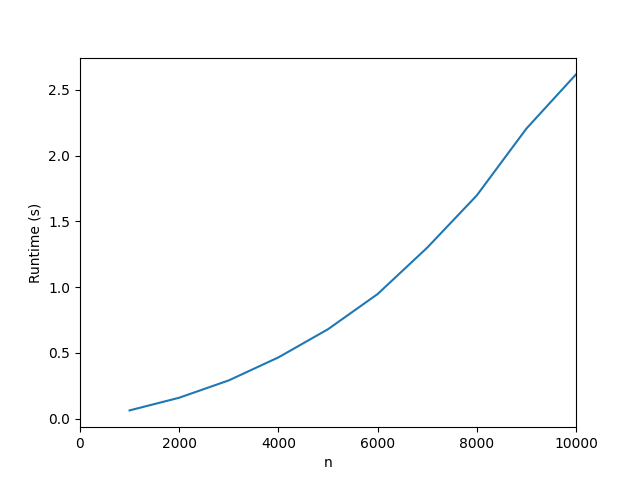
\includegraphics[scale=0.65]{iterative}

    This indeed appears to be an approximately linear relation.

    These runtimes cannot be compared to the naive implementation's runtimes
    since the values for $n$ are very different,
    besides the obvious fact that $n = 20$ for the naive implementation
    is slower than $n = 10000$ for the iterative implementation.


    \subsection*{The Binary Exponentiation Implementation}

    Consider
    \[
        \mathbf{v}_k =
        \begin{bmatrix}
            S(2k + 1) \\
            S(2k + 2)
        \end{bmatrix}
    \]
    as a 2D vector (where $k = \left\lfloor \frac{n - 1}{2} \right\rfloor$).
    Then,
    \begin{align*}
        \mathbf{v}_{k + 1} &=
        \begin{bmatrix}
            S(2k + 3) \\
            S(2k + 4)
        \end{bmatrix}
        \\
        &=
        \begin{bmatrix}
            2 * S(2k + 2) - S(2k + 1) \\
            S(2k + 3) + S(2k + 2)
        \end{bmatrix}
        \\
        &=
        \begin{bmatrix}
            2 * S(2k + 2) - S(2k + 1) \\
            3 * S(2k + 2) - S(2k + 1)
        \end{bmatrix}
        \\
        &= M \mathbf{v}_k
    \end{align*}
    where
    \[
        M =
        \begin{bmatrix}
            -1 & 2 \\
            -1 & 3
        \end{bmatrix}
    \]
    Then, since
    \[
        \mathbf{v}_0 =
        \begin{bmatrix}
            1 \\
            2
        \end{bmatrix}
        \qquad
        \text{and}
        \qquad
        \mathbf{v}_k = M^k \mathbf{v}_0
    \]
    we can evaluate using binary exponentiation on the matrix.

    Binary exponentiation takes $O(\log k) = O(\log n)$ time.

    The runtimes for $n \in \{1000, 2000, \dots, 10000\}$
    when run $1000$ times each make the following plot:

    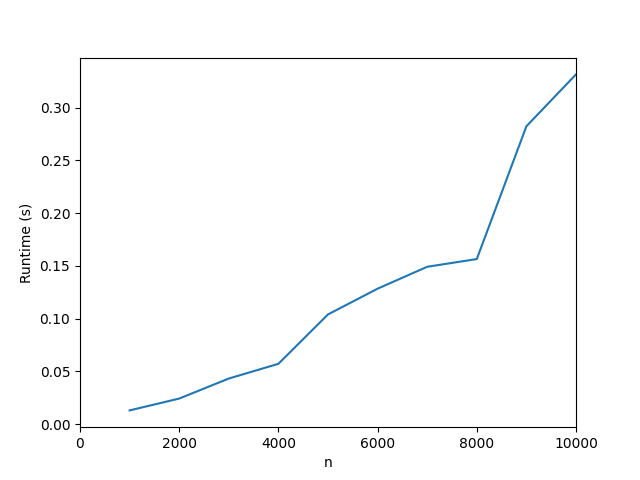
\includegraphics[scale=0.65]{binary}

    This does not look quite like logarithmic time complexity,
    but it also is so fast that random noise seems to have a significant effect,
    and it quickly finds such large numbers that large integer multiplication
    costs might play a role.
    At the very least it is two orders of magnitude faster than the iterative algorithm.

\end{document}